%!TEX root=../book.tex

\chapter{Alternatives to \textit{t}-Tools}

\section{What Are Nonparametric Statistics?}

Nonparametric statistics \index{Nonparametric statistics} are those that are not based on paramaterized probability distributions. Did that lose you? That's okay if you're scratching your head.

The idea is that most test rely on parameters such as mean, variance, etc. (Thus, this family of procedures is known as parametric statistics.) When we're talking about nonparametric statistics, we mean that we aren't making assumptions about the data belonging to any particular distribution.

Let's take \textit{t}-tools from the previous chapter: those rely on sample means taken from two populations that we assume to be normally distributed. If those populations don't follow this distribution, our test can fall apart and give us misleading results.

With nonparametric tests, our data don't need to follow any particular distribution: our statistical tests are agnostic to this. We are able to achieve this break from dependence on probability distribution in one of two ways: through distribution-free statistical methods and through nonparametric statistics.

In either case, nonparametric tests will usually operate on ordinal data: that is, data that are numeric, but that don't have any true 0 or necessarily equal spacing between items. For instance, if we were administering a health survey and asked respondents, "How would you rate your current health?"

Although the options might be ``excellent,'' ``good,'' ``average,'' ``poor,'' or ``one foot in the grave,'' for research purposes, they would be coded 1 through 5, respectively. Although we know that 1 means the respondent thinks he or she is in excellent health, the number itself doesn't signify anything meaningful: there is no meaningful 0 on this scale, and we don't know if the difference between a 1 and a 2 is the same as the difference between a 2 and a 3.

\section{Overview of Nonparametric Tools for Two Samples}

Although there are many types of nonparametric tests, we will only go over one or two right now. If it doesn't look like these are quite right for your needs, check out our chapter later on in the book on working with rank-ordered data: there we give a more general overview of nonparametric tests beyond only the context of a two-sample comparison.

\subsection{Man-Whitney U Test}

First up is the Mann-Whitney U test \index{Mann-Whitney U test}, also variously known as the Mann-Whitney-Wilcoxon \index{Mann-Whitney-Wilcoxon test} test, the Wilcoxon rank-sum test \index{Wilcoxon rank-sum test}, and the Wilcoxon-Mann-Whitney test \index{Wilcoxon-Mann-Whitney test}. Whew, that's a mouthful.

Thankfully, though, the test itself is a bit simpler than deciding what to call it! The basic idea here is that we are going to take the data from our two samples and rand-order them. For example, let's say that we're working in a call center and we launch a campaign to decrease customers' wait time before they are connected to a representative. We measure the wait times both before and after this campaign and want to determine whether there was an impact of the initiative.

To test this, we will (1) combine the data from the two samples; (2) rank all of the values in ascending order; (3) calculate the ranks for ties (by averaging the rank of each tied item); and (4) calculate the sum of the ranks for the first sample (in this example, the wait times before our intervention). Our process might look something like this:

\begin{tabular}{r | l l l}
Condition & Wait time (mins) & Rank & Tied rank \\
\hline
Before & 0.1 & 1 & 1.5 \\
After & 0.1 & 2 & 1.5 \\
After & 0.1 & 3 & 1.5 \\
Before & 0.2 & 4 & 4 \\
Before & 0.3 & 5 & 5.5 \\
Before & 0.3 & 6 & 5.5 \\
After & 0.4 & 7 & 7 \\
Before & 0.5 & 8  & 8 \\
\vdots & \vdots & \vdots & \vdots \\
After & 17.2 & 152 & 152 \\
After & 17.8 & 153 & 153 \\
Before & 17.9 & 154 & 154 \\
After & 18.0 & 155 & 155.5 \\
Before & 18.0 & 156 & 155.5 \\
Before & 18.1 & 157 & 157 \\
After & 18.2 & 158 & 158 \\
Before & 18.4 & 159 & 159 \\
\hline
\multicolumn{3}{l}{Sum of ranks for Before Intervention} & $9743.5$ \\
\end{tabular}

So, here we have our indicator variable in the first column, our raw data in the second column, ordered from smallest to largest, and our ranked values in the third and fourth columns. Again, whenever we have a tie, we take the average rank of all tied items at that measurement. Finally, we take all of the ranks for our ``Before Intervention'' and add them up to get our W statistic.

And, at last, we're ready to go and conduct our fun little statistical test. To do this, we'll use the formula (it's a doozy!):
\begin{equation}
Z_W = \frac{\left|W-\frac{n(m+n+1}{2}\right|-0.5}{\sqrt{\frac{mn(m+n+1)}{12}}}
\end{equation}
where $W$ is the Mann-Whitney test statistic that we calculated above, $n$ is the size of the first sample, and $m$ is the size of the second sample. Of course, this is only unless there are ties, in which case the equation gets even funkier. But it's all good! Modern statistical packages have you covered: no chance we're about to make you do this all by hand.

The point is, this ends up spitting out a handy $Z_W$ statistic and \textit{p}-value, real similar to a \textit{t}-test like the ones we just ran.

\subsection{Wilcoxon Signed Rank Test}

Despite the similarity in names, this is actually an entirely separate test from the one that we just ran (although if you didn't already guess it, we're going to be doing some more ranking!).

In this test, we compute what's called a signed rank (so it's a signed rank test! Such creative names\ldots). It's a pretty similar procedure to the previous test, but differs in that we are working with paired values whereas the previous test is more analogous to an independent-samples \textit{t}-test. Given this, we compute a difference score between the pre- and post-test values.

Let's take the example of a high school math test: a teacher wants to find out if a review session helps her students' understanding of the concepts they've covered in the last chapter. To test this, she administers a pretest and computes each student's percentage score, gives the lesson, and then conducts a post-test and computes students' percentage scores again.

For the purposes of this test, we will rank the scores based on the magnitude of their difference. For instance:

\begin{tabular}{l l l | c c c c}
Student & Pre & Post & Difference & Magnitude & Rank & Signed rank \\
\hline
1 & 78 & 78 & 0 & 0 & --- & --- \\
2 & 80 & 78 & 2 & 2 & 1 & 1 \\
3 & 81 & 84 & -3 & 3 & 2 & -2 \\
4 & 68 & 72 & -4 & 4 & 3 & -3.5 \\
5 & 84 & 80 & 4 & 4 & 4 & 3.5 \\
6 & 90 & 98 & -8 & 8 & 5 & -5 \\
\vdots & \multicolumn{2}{c}{\vdots} & \multicolumn{2}{c}{\vdots} & \multicolumn{2}{c}{\vdots} \\
\end{tabular}

Here we (1) order the data by the magnitude of their differences; (2) rank those data; (3) compute the average rank for tied values; and (4) include the sign of the original difference (i.e., whether the difference is positive or negative). Then we add up all of the signed rank values  to compute  an  overall  $W$  statistic.

Following  that,  there's  another  formula that's  just  as  fun  as the  last  one---so  fun in fact that we aren't even going to include  it here!  What's important  is that once again you get a $Z$ statistic and \textit{p}-value at the  end of  it  all.

\section{Cautions and Considerations}

\subsection{Assumptions of the Mann-Whitney Test}

This test assumes that:
\begin{enumerate}
\item all observations are independent of one another;
\item the data are measured on an ordinal scale;
\item the distributions of both groups are equal under the null hypothesis;
\item the responses are continuous; and
\item the alternative hypothesis is restricted to a shift in location (i.e., $F_1(x)=F_2(x+\delta)$).
\end{enumerate}

\subsection{Assumptions  of  the Wilcoxon Signed-Rank Test}

This test assumes:
\begin{enumerate}
\item data are paired and come from the same population;
\item each pair is chosen randomly;
\item each pair is independent of every other pair; and
\item the data are measured on an ordinal scale.
\end{enumerate}

\section{Implementation in R}

Please note: all data used in these explanations are simulated. For both tests, the same function, \verb|wilcox.test(x,y)| is called. One important tidbit to remember is that the default function does not handle ties gracefully. If you have any ties in your data, you should instead use \verb|wilcox_test()| in the \verb|coin| package. We detail the use of both below.

\subsection{Mann-Whitney Test}

To specify that a Mann-Whitney test should be conducted, we set the \verb|paired| flag to \verb|FALSE|:

\begin{framed}
\begin{Verbatim}[samepage=TRUE]
set.seed(0)
before <- c(rnorm(100, 4.9, 3.8))
after <- c(rnorm(100,3.8, 2.9))

wilcox.test(before, after, paired = FALSE)
\end{Verbatim}
\end{framed}

\subsection{Wilcoxon Signed-Rank Test}

This test can be conducted with either two vectors of paired data or a single vector of difference values (i.e., $x_1-x_2$). For both tests, we indicate that a Wilcoxon signed-rank test should be conducted by setting the \verb|paired| flag to \verb|TRUE|.

\begin{framed}
\begin{Verbatim}[samepage=TRUE]
set.seed(0)
pretest <- c(rnorm(100,70,10))
posttest <- c(rnorm(100,85,7))
difference <- pretest - posttest

# Paired-samples test
wilcox.test(pretest, posttest, paired = TRUE)

# Difference vector or one-sample test
wilcox.test(difference, paired = TRUE)
\end{Verbatim}
\end{framed}

\section{Case Study: Heavy Metal Accumulation}

In 2004, \href{http://www.sciencedirect.com/science/article/pii/S0269749104001058}{Laureysensa, et al.} looked at the ability of a number of poplars to resorb heavy metals from the soil in which they were planted. Specifically, they were interested in looking at seasonal variation in these resorption patterns: whether the poplars would more actively take up heavy metals from the soil during certain times of the year than others.

To this end, they looked at the resorption patterns of 13 different cloned poplars for aluminum, cadmium, iron, manganese, and zinc and measured their heavy metal content ($\mu g/g$) in both August and November of the same year. However, due to oddities of the data, a typical parametric test to look at seasonal differences might not be appropriate. Rather, we will use Wilcoxon's signed rank test.

For this study, let's focus only on one of the heavy metals measured: aluminum. We can start by visualizing the distributions of both samples (Figure \ref{fig:tAlt01}).

\begin{figure}[htp]
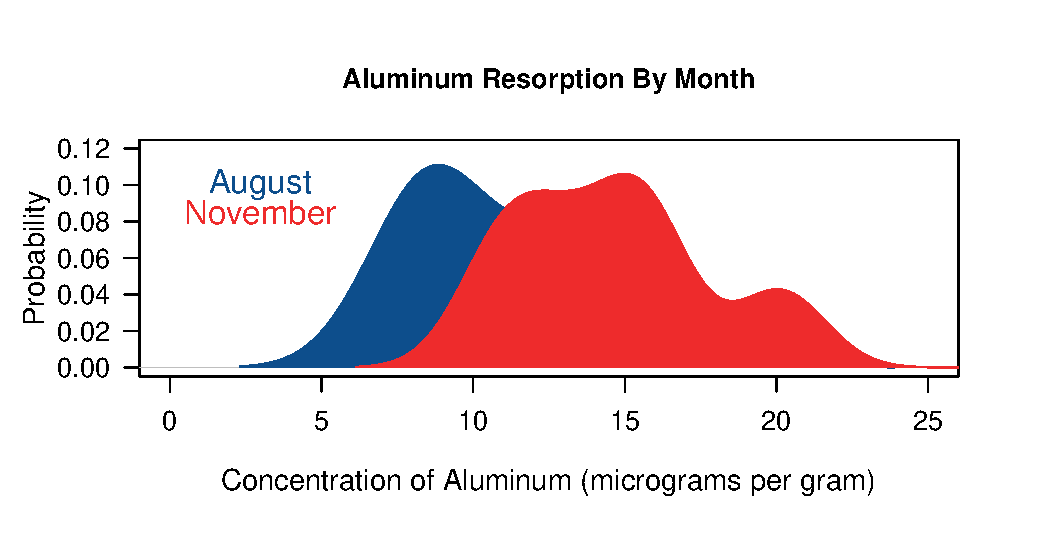
\includegraphics[width=35pc]{tAlternative01}
\caption{}
\label{fig:tAlt01}
\end{figure}

As we can see, their probability densities differ somewhat from one another and both depart from the normal distribution. Given this, we can assume that a \textit{t}-test may not be most appropriate to judge the differences between these two samples.

Knowing that, we can construct our null and alternative hypotheses for these data:
\begin{eqnarray*}
H_0:& \tilde{\mu}_{\text{aug}} = \tilde{\mu}_{\text{nov}} \\
H_A:&  \tilde{\mu}_{\text{aug}} \neq \tilde{\mu}_{\text{nov}} \\
\end{eqnarray*}
where $\tilde{\mu}$ is the median for each sample. We then conduct a Wilcoxon signed rank test to evaluate these hypotheses:

\begin{framed}
\begin{Verbatim}[samepage=TRUE]
	Wilcoxon signed rank test

data:  august and november
V = 16, p-value = 0.03979
alternative hypothesis: true location shift is not equal to 0
\end{Verbatim}
\end{framed}

This test indicates that the the medians of the two samples do differ to a level of statistical significance, $V = 16$; $p\text{-value}=0.040$, indicating that resorption of aluminum among poplars is more efficient during the winter months ($\tilde{x}=15.3$) than during the fall ($\tilde{x}=10.0$).

\section{Exercises}

\section{Additional Resources}

